\documentclass[a4paper
,12
,twocolumn
]{article}

\usepackage[dvipdfm]{hyperref}
\hypersetup{
  setpagesize=false,
  bookmarksnumbered=true,
  colorlinks=true,
}

\hypersetup{
  pdfstartview={FitV},
  pdftitle={WiredTiger Backend for OpenLDAP},
  pdfauthor={Open Source Solution Technology Corporation HAMANO Tsukasa \textless{}hamano@osstech.co.jp\textgreater{}},
  pdfsubject={},
  pdfkeywords={},
}

\usepackage[dvipdfmx]{color}
\usepackage[dvipdfmx]{xcolor}
\usepackage[dvipdfmx]{graphicx}
\usepackage{here}

% title
\title{WiredTiger Backend for OpenLDAP}
\author{Open Source Solution Technology Corporation \\ HAMANO Tsukasa \textless{}hamano@osstech.co.jp\textgreater{}}
\date{\today}

\makeatletter
\def\@maketitle{
  \newpage
  \null
  \begin{center}
    {\LARGE \@title \par}
  \end{center}
  \smallskip
  \begin{flushright}
    {\large \@author \par}
    {\large \@date \par}
  \end{flushright}
  \vspace{0.5in}
}
\makeatother

% document
\begin{document}
\maketitle
\abstract{This paper introduces WiredTiger backend for OpenLDAP. WiredTiger is an
embedded database having the characteristics of multi-core scalability
and lock-free algorithms. We implemented a new OpenLDAP backend called
back-wt that is using WiredTiger database and then measured the
performance.}
\section{Motivation}\label{motivation}

BerkeleyDB is a legacy embedded database. The write performance of
back-bdb(OpenLDAP backend using BerkeleyDB) is painfully slow and not
scalable. If we use asynchronous mode in order to improve the write
performance, data durability will be sacrificed. The WiredTiger backend
will bring about high write performance and high concurrency performance
for OpenLDAP.

\section{Data Structure}\label{data-structure}

First, we had to choose data structure either plain structure such as
back-bdb or hierarchical structure such as back-hdb. If we choose the
plain structure, sub scope search is fast but modrdn and add operations
need some cost. The plain structure need many \texttt{@prefix} entries
for sub scope search, and also \texttt{\%prefix} entries are needed. If
we choose the hierarchical structure, modrdn is fast but lookup and add
operations need some cost.

\begin{figure}[H]
\centering
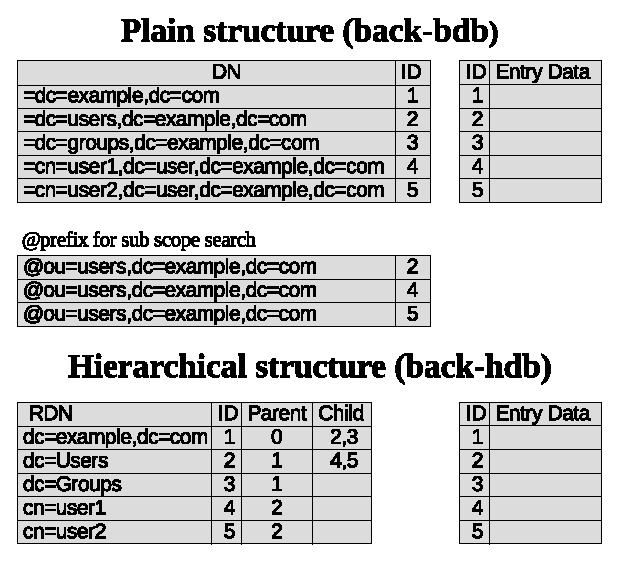
\includegraphics[width=0.9\columnwidth]{figure/plain_vs_hierarchical.eps}
\caption{Plain structure vs Hierarchical structure}
\end{figure}

We followed basically plain data structure but we made some enhancements
to the data structure for performance and database footprint. Before
adding an entry, we reversed the DN per RDN and then added the
\texttt{Reverse\ DN} as the key into WiredTiger's B-Tree table. At this
point, entries are sorted by \texttt{Reverse\ DN}, So we can search
rapidly with a sub scope using WiredTiger's range search. The range
search method is low cost that only needs
\texttt{WT\_CURSOR::search\_near()} and increment cursor operations for
this purpose.

\begin{figure}[H]
\centering
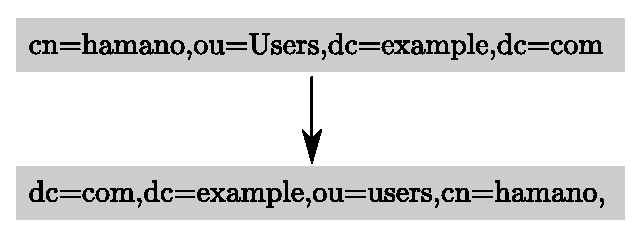
\includegraphics[width=0.9\columnwidth]{figure/reverse_dn.eps}
\caption{Making Reverse DN}
\end{figure}

\begin{figure}[H]
\centering
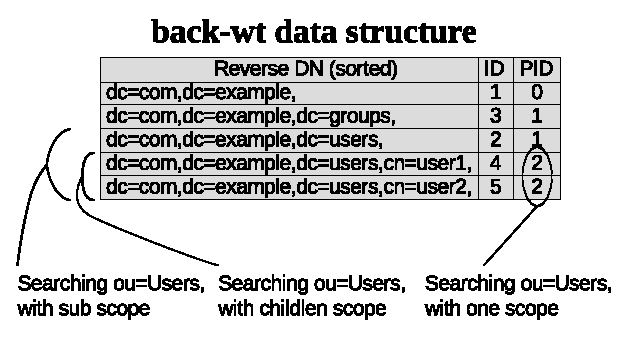
\includegraphics[width=0.9\columnwidth]{figure/back-wt_data_structure.eps}
\caption{back-wt data structure}
\end{figure}

\section{Current Status}\label{current-status}

\begin{itemize}
\itemsep1pt\parskip0pt\parsep0pt
\item
  slapadd, slapcat, slapindex have been implemented.
\item
  LDAP BIND, ADD, DELETE and SEARCH have been implemented.
\item
  MODIFY and MODRDN have not been not implemented yet.
\item
  deref search has not been implemented yet.
\item
  WiredTiger does not support multiprocess access yet. It means that we
  can't do slapcat while running slapd at the moment. However,
  WiredTiger is planning to support RPC in the future. If it is
  realized, we can do hot-backup while avoiding multi-process locking.
\item
  We do not implement entry cache similar to back-bdb. It's not
  absolutely necessary since WiredTiger cache is fast enough.
\end{itemize}

\section{Benchmarking}\label{benchmarking}

We have measured benchmarks that focus on concurrency performance. We
use benchmarking tool called lb.\footnote{\url{https://github.com/hamano/lb}}
See our wiki page for detail of benchmarks.\footnote{\url{https://github.com/osstech-jp/openldap/wiki/back_wt-benchmark}}

\begin{figure}[H]
\centering
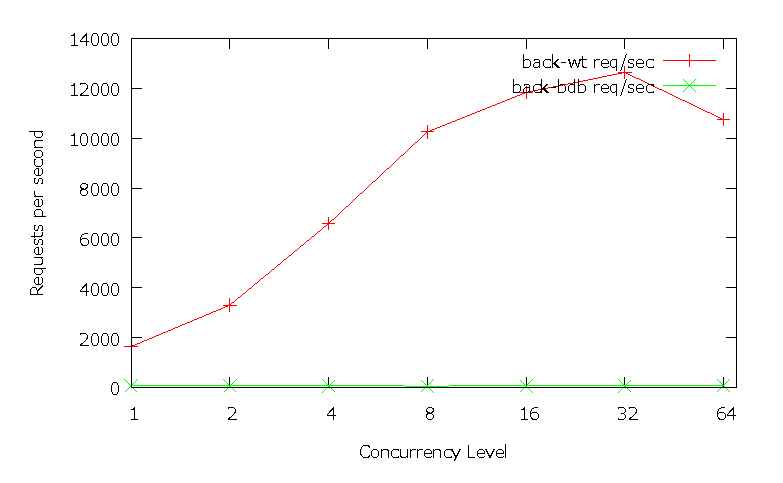
\includegraphics[width=0.9\columnwidth]{benchmark/add.eps}
\caption{LDAP ADD Benchmarking}
\end{figure}

\begin{figure}[H]
\centering
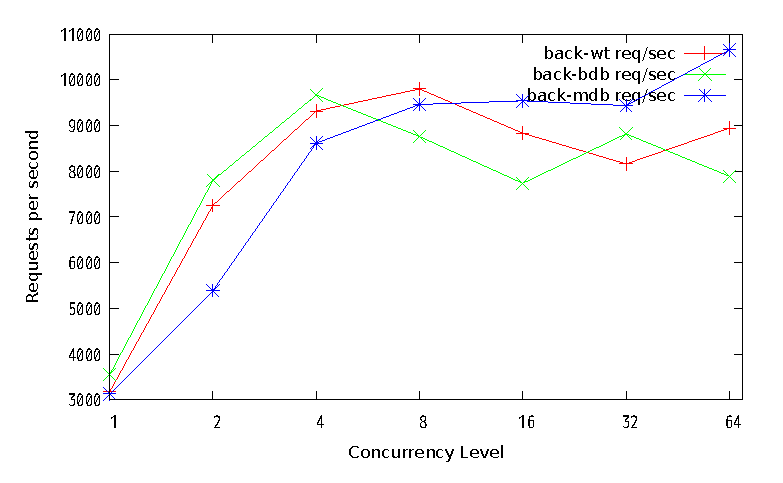
\includegraphics[width=0.9\columnwidth]{benchmark/bind.eps}
\caption{LDAP BIND Benchmarking}
\end{figure}

\begin{figure}[H]
\centering
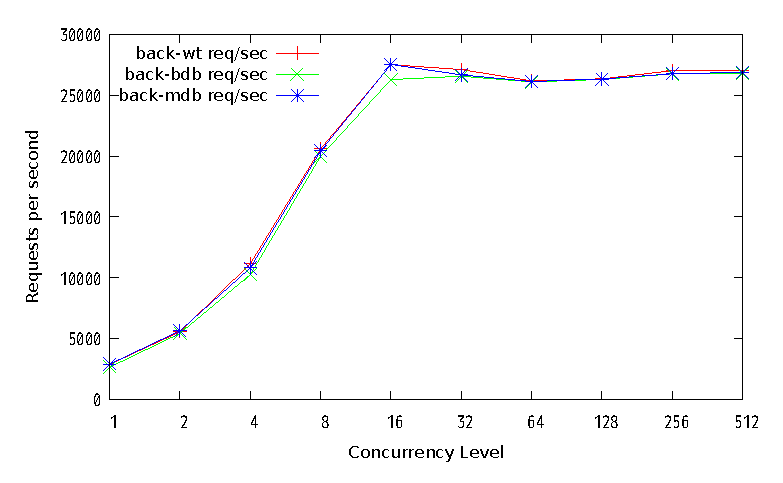
\includegraphics[width=0.9\columnwidth]{benchmark/search.eps}
\caption{LDAP SEARCH Benchmarking}
\end{figure}

\subsection{Analysis}\label{analysis}

\begin{itemize}
\itemsep1pt\parskip0pt\parsep0pt
\item
  We used 2x6-Core CPU(24-Hyper-Threading). We may get more scalability
  on more CPUs.
\item
  The ADD graph is not broken. back-wt is faster overwhelmingly.
\item
  The read performance is same level. However, it is necessary to
  consider that we did not implement entry cache to back-wt.
\end{itemize}

\end{document}
